
\section{Algorithm explanation}

\subsection{AKAZE}

AKAZE is an \textbf{Accelerated} version of KAZE\@. It's faster because it builds
it's nonlinear scale space representation using a mathematic framework called
Fast Explicit Diffusion. It has the following steps:
\begin{easylist}[tractatus]

# Building a Nonlinear Scale Space with Fast Explicit Diffusion

## We first need the contrast factor \(\lambda\), which we get from an
algorithm defined in the AKAZE paper. That algorithm uses a gaussian smoothed
input image.

## The next step is to run the FED cycles, which are explicit diffusion schemes
with varying time steps.

### In AKAZE, the FED scheme is embedded in a fine to coarse pyramidal approach
which increases computation speed and results in a set of filtered images.

# Feature Detection

## Compute the determinant of Hessian using the set of filtered images obtained
from the previous step.

# Feature Description

## AKAZE uses a Modified-Local Difference Binary (M-LDB) descriptor. 

### The descriptor uses gradient and intensity information from the nonlinear
scale space.

\end{easylist}

\subsection{LIOP}

\begin{figure}
  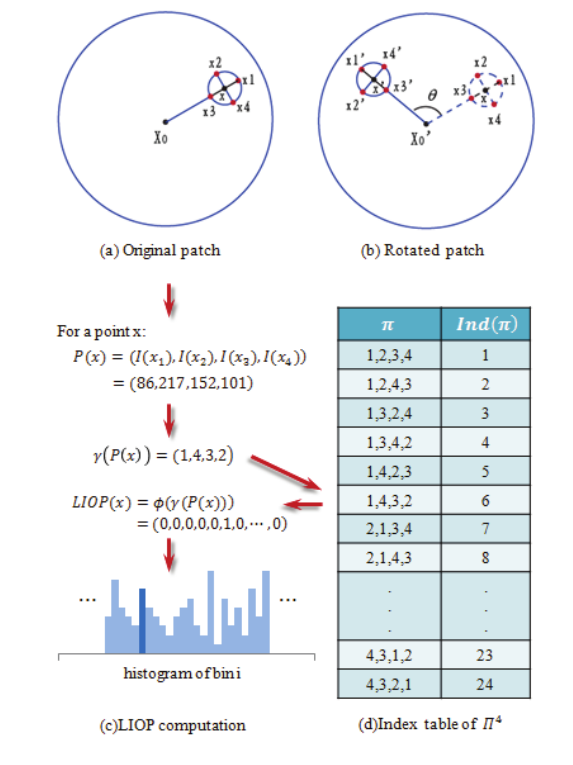
\includegraphics[width=\textwidth]{liop_descriptor}
  \caption{The LIOP descriptor, taken from the LIOP paper.}
\label{fig:liop_descriptor}
\end{figure}

\NewList{}
\begin{easylist}[tractatus]

  # Pre-processing, Feature Detection and Normalization

  ## The input image is smoothed with a Gaussian filter.

  ## An affine covariant detector is run to localize the features and estimate
  the affine shapes of their neighborhoods.

  ## The detected regions are normalized to circular regions.

  ## The image is smoothed a again with a Gaussian filter to remove noise from
  the normalization step.

  # Region Division

  ## The output from the previous step is divided into subregions, according to
  their intensity.

  # Local Intensity Order Pattern Descriptor

  ## The LIOP is calculated for each point in a subregion.

  ## After that the LIOPs in each subregion are combined to create the
  descriptor.

  ### Figure~\ref{fig:liop_descriptor} has a graphical representation of the
  descriptor.

\end{easylist}

\subsection{OIOP}

OIOP is based on LIOP, and many of the steps are the same.

\NewList{}
\begin{easylist}

  # Intensity Order Based Patch Division

  ## Like in LIOP, an affine covariant detector is used to localize a keypoint
  and estimate the affine shape of its neighborhood.

  ## The resulting area is then normalized to a circle, and smoothed with a
  Gaussian filter. The resulting region is called a patch.

  ## Like in LIOP, the patch is divided into subregions or bins according to
  their intensity.

  ## A descriptor is created by constructing a low-level descriptor seperately
  for each bin, and concatenating the resulting descriptors.

  # Local Intensity Order Pattern

  ## Create the LIOP descriptor
 
  # Overall Intensity Order Pattern

  ## The problem with LIOP is that because it uses neighbor points' intensity
  order, it is not robust to noise. OIOP intends to solve this by taking the
  overall intensity distribution in the patch to account.

  ## This is done by quantizing the neighbor points' intensity, which
  effectively lessens the effect of noise on the intensity.

  ## The quantizing can also be learning-based, which increases the
  adaptability of the algorithm.

\end{easylist}

\section{Answers to given questions}

\subsection{Explain the difference between SIFT and A-KAZE for detecting local
maxima.}

SIFT tries to detect local maxima from linear Gaussian scale space. Linear
scale-space has the disadvantage that the whole image is blurred. A-KAZE uses
non-linear scale space, which preserves the strong edges of the image, while
still removing noise.

\subsection{Explain the difference between LIOP and OIOP descriptors.}

The LIOP descriptor only takes into account the exact intensity between the
sampling points. This makes it sensitive to noise, for example. The OIOP
accounts for this by coarsely quantizing the intensity values of the points.
In standard quantization, the quantization is based on a manually set
constant. In learning based quantization the amount of quantization can be
learned, thus increasing adaptability.

\subsection{As we can see in (2), LIOP descriptor is rotation-invariant by
itself.  Explain the technical reason of the property.}

The descriptor consists of the keypoint and its neighbors, ie.\ points
around it.  The neighbors are distributed equally in a circle around the
keypoint. The first neighbor to be sample is along a line that goes from
the center of the patch to the keypoint. As the neighbors are equally
distributed, there are two neighbors on this line. The furthest from the
center point is the first to be sampled. The other neighbors are sampled
anticlockwise from the first point.

The descriptor is rotation invariant because this grouping of points retain
their relation to each other and the patch no matter the rotation. This
might be understood more clearly from the figure~\ref{fig:liop_descriptor}.








